\section{図・表の配置}

\subsection{図の自動配置}
\label{sec:allocate_fig}

\code\ref{code:fig_env}において,figure環境を用いた図の表示方法を説明した.
ただし,\code\ref{code:fig_env}の記述方法では図が意図した位置に表示されないことも多い.
そこで,\textbackslash begin\{figure\}のオプションで位置指定を行う.
位置指定に使用できる文字は以下のとおりである.
\begin{itemize}
  \item t:ページ上端(top)に図を出力する
  \item b:ページ下端(bottom)に図を出力する
  \item p:単独ページ(page)に図を出力する
  \item h:できればその位置(here)に図を出力する
\end{itemize}

これらの位置指定オプションは\textbackslash begin\{figure\}[tbph]のように記述して指定する.
このような記述の場合,tでうまく表示できないときにはb,bでうまく表示できないときはpのように,4つの位置指定をその順にうまく表示できるか試行する.
なお,tbpやtbのように一部の文字だけを用いた位置指定でも問題ない.

また,[b!]のように指定すると,[b]よりもより強い指定となる.
さらに,プリアンブルにおいて,\textbackslash usepackage\{float\}と記述して,floatパッケージを取り込むと,[H]のような記述をすることもできる.
この[H]という記述によって,必ずその位置に図を出力するという指定を行うことができる.

\subsection{表の自動配置}

表においても同様である.
\code\ref{code:table_env}の記述方法では表が意図した位置に表示されないことが多いため,\ref{sec:allocate_fig}と同じ位置指定オプションを\textbackslash begin\{table\}のオプションで設定する.

\subsection{左右に並べる配置}

場合によっては複数の画像や表を横並びで表示させたいこともあろう.
その場合は\code\ref{code:minipage_env}のように,minipage環境を用いる.
minipage環境は,\textbackslash begin\{minipage\}\{$\cdots$\}の$\cdots$の部分に記述した幅に合わせた小さなページを作り,その中に図を配置することによって,左右横並びに図を出力させることを可能にする.
指定する幅の大きさによっては,図を横に3枚や4枚並べることも可能になる.

幅の指定はmm等の環境に依存しない指定方法もあるが,\code\ref{code:minipage_env}では,\textbackslash linewidthを用いた環境依存の指定方法を使用している.
\textbackslash linewidthは現在の環境\footnote{記述位置によって異なる.すなわち,\textbackslash begin\{itemize\}と \textbackslash end \{itemize\}の間に書けば, itemize環境が現在の環境である.}の幅に合わせることが可能である.
\code\ref{code:minipage_env}において,0.4\textbackslash linewidthと記述しているのは,minipageの環境の幅を,現在の環境の幅\footnote{ここではdocument環境の幅,すなわち,文章の幅である.}の0.4倍とするためである.
ちなみに,\textbackslash includegraphicsのオプションで,width=\textbackslash linewidthと記述しているが,これは,画像の幅をminipage環境\footnote{これが現在の環境になっている}の幅に合わせるための記述である.

また,複数の図を並べて配置した場合に,それらの下部にキャプションをつけたい場合はsubcaptionパッケージを取り込みが必要である.
プリアンブルにおいて,\textbackslash usepackage\{subcaption\}を記述したうえで,\textbackslash subcaption\{$\cdots$\}にそのキャプションを記述する.

\begin{lstlisting}[caption=minipage環境を使用した配置,label=code:minipage_env]
  \documentclass{jsarticle}
  \usepackage[dvipdfmx]{graphicx}
  \usepackage{subcaption}

  \begin{document}
  
  \begin{figure}[tbph]
    \centering
    \vspace{4mm}
    \begin{minipage}{0.4\linewidth}
        \centering
        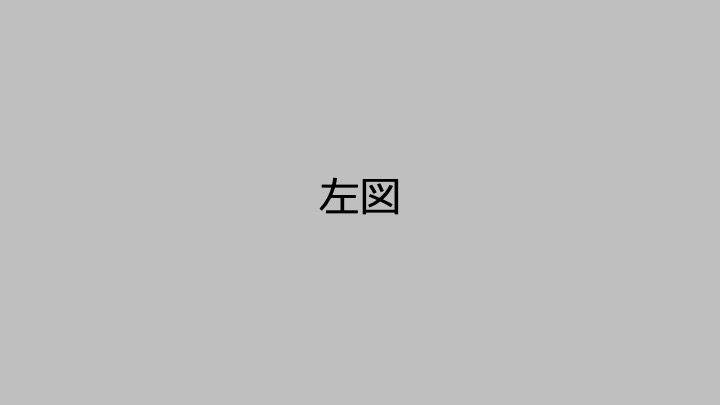
\includegraphics[width=\linewidth]{fig_left.jpeg}
        \subcaption{ひだりのきゃぷしょん}
        \label{fig:fig_left}
    \end{minipage}
    \hfill
    \begin{minipage}{0.4\linewidth}
        \centering
        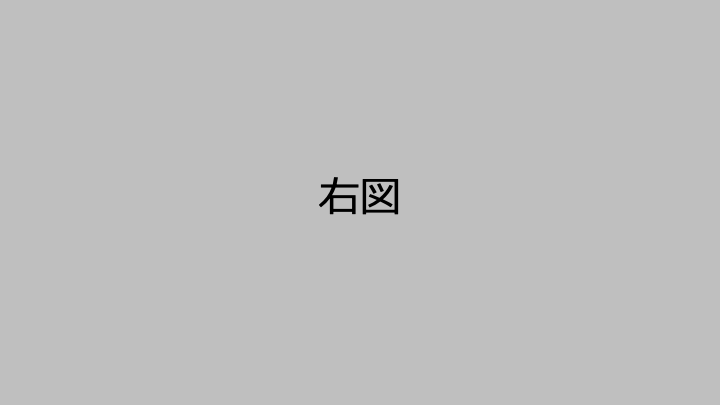
\includegraphics[width=\linewidth]{fig_right.png}
        \subcaption{みぎのきゃぷしょん}
        \label{fig:fig_right}
    \end{minipage}
    \caption{きゃぷしょん}
  \end{figure}

  \end{document}
\end{lstlisting}

\code\ref{code:minipage_env}は以下のように出力される.

\noindent\textbf{出力結果:}\hrulefill\\
\vspace{-6mm}
\begin{figure}[tbph]
  \centering
  \vspace{4mm}
  \begin{minipage}{0.4\linewidth}
      \centering
      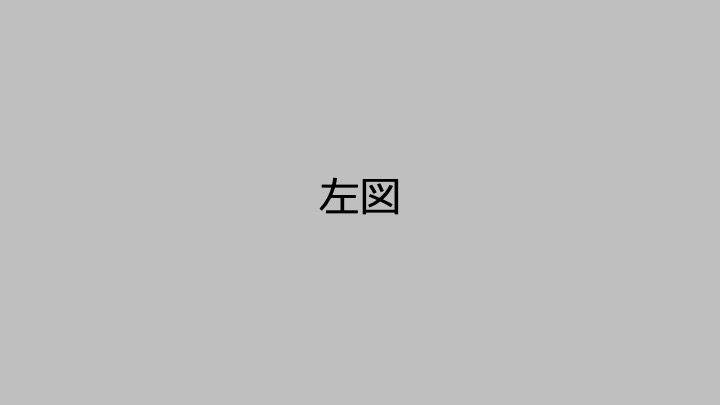
\includegraphics[width=\linewidth]{fig_left.jpeg}
      \subcaption{ひだりのきゃぷしょん}
      \label{fig:fig_left}
  \end{minipage}
  \hfill
  \begin{minipage}{0.4\linewidth}
      \centering
      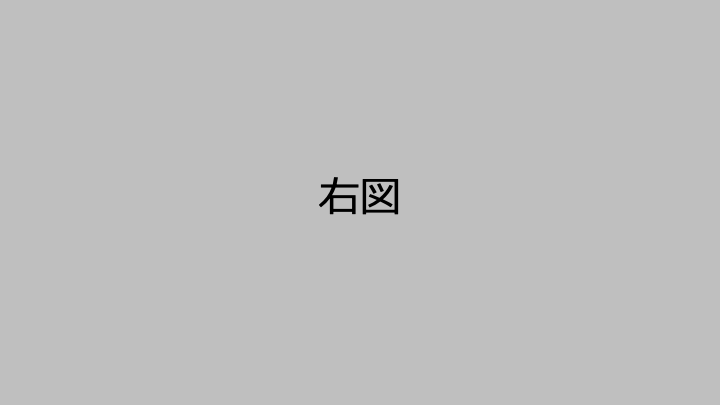
\includegraphics[width=\linewidth]{fig_right.png}
      \subcaption{みぎのきゃぷしょん}
      \label{fig:fig_right}
  \end{minipage}
  \caption{きゃぷしょん}
\end{figure}
\\\noindent\hrulefill  

